% =============================================================================
%  PARTE 0 — INTRODUÇÃO: PREFÁCIO DO AUTOR, GÊNESE DO ECOSSISTEMA,
%  COMO USAR ESTE LIVRO E VISÃO PANORÂMICA
%  Autor: Marcelo Claro Laranjeira
% =============================================================================
\chapter*{Introdução ao Ecossistema}
\addcontentsline{toc}{chapter}{Introdução ao Ecossistema}
\setcounter{chapter}{1}
\label{ch:introducao}

% =============================================================================
%  SEÇÃO 1: INTRODUÇÃO FORMAL COM RIGOR CIENTÍFICO
% =============================================================================
\section{Introdução}

\paragraph*{Contexto e Problema de Pesquisa.}
A engenharia de software contemporânea enfrenta um paradoxo fundamental:
embora as ferramentas de desenvolvimento tenham atingido níveis
extraordinários de sofisticação, o processo de produção de software
permanece intrinsecamente artesanal \cite{brooks1995mythical}.
Cada funcionalidade, correção ou refatoração demanda atenção humana
dedicada, estabelecendo um gargalo que a computação tradicional não
consegue superar: a \destaque{atenção humana} é o recurso mais escasso
no ciclo de desenvolvimento \cite{endres2003software}.

Sistemas multiagentes (MAS) surgiram como uma alternativa promissora para
automatizar não apenas tarefas isoladas, mas fluxos de trabalho complexos
que exigem coordenação e adaptação \cite{wooldridge2009multiagent}.
Plataformas como LangChain,\footnote{\textit{LangChain} é um framework de
orquestração de LLMs que encadeia chamadas a modelos de linguagem em
pipelines sequenciais. Diferencia-se do \opencodeeco{} por não possuir
mecanismos de metacognição ou auto-evolução.} CrewAI,\footnote{\textit{CrewAI}
é uma plataforma multiagente declarativa onde papéis (\textit{roles}) são
definidos estaticamente. Ver Capítulo~\ref{ch:comparacao} para uma análise
comparativa detalhada.} e AutoGPT \cite{significantgravitas2025autogpt}
demonstraram a viabilidade técnica da orquestração autônoma, mas
revelaram limitações críticas: rigidez arquitetural, incapacidade de
auto-diagnóstico e ausência de mecanismos formais de confiança entre
agentes \cite{xi2023rise}.

O \opencodeeco{} foi concebido para endereçar exatamente essas limitações,
propondo um ecossistema integrado onde agentes não apenas executam
tarefas, mas monitoram, diagnosticam e evoluem seu próprio comportamento
por meio de um pipeline epistemológico composto por seis scanners
formais\footnote{O pipeline epistemológico compreende: Scanner Noológico
(SPEC-028), Scanner Teleológico (SPEC-029), Scanner Evolutivo (SPEC-030),
Scanner de Refinamento (SPEC-031), MCSP (SPEC-032) e Potentiality Scanner
(SPEC-043). Cada scanner opera em um nível distinto de abstração,
conforme detalhado no Capítulo~\ref{ch:scanners}.} e um motor de confiança
comportamental (Trust Engine, SPEC-038).

\begin{figure}[htb]
\centering
\caption{Quatro pilares teóricos do OpenCode Ecosystem}
\label{fig:quatro-pilares}
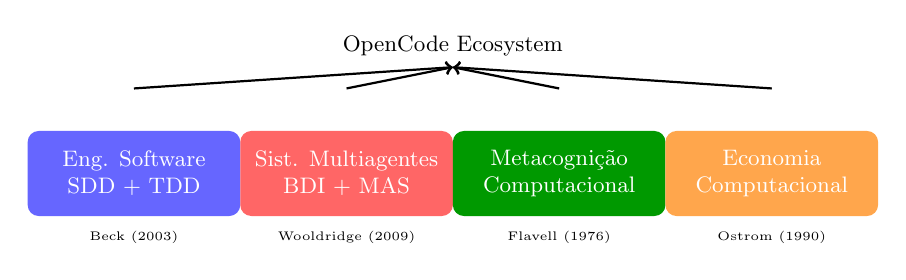
\begin{tikzpicture}[scale=0.9, every node/.style={scale=0.9}]
  \tikzstyle{pilar}=[rectangle, rounded corners, minimum width=3cm, minimum height=1.2cm,
                     align=center, font=\small, text=white]
  \node[pilar, fill=blue!60] at (-4.5,0) {Eng. Software\\SDD + TDD};
  \node[pilar, fill=red!60] at (-1.5,0) {Sist. Multiagentes\\BDI + MAS};
  \node[pilar, fill=green!60!black] at (1.5,0) {Metacognição\\Computacional};
  \node[pilar, fill=orange!70] at (4.5,0) {Economia\\Computacional};

  \node[font=\small] at (0,1.8) {OpenCode Ecosystem};
  \draw[->, thick] (-4.5,1.2) -- (0,1.5);
  \draw[->, thick] (-1.5,1.2) -- (0,1.5);
  \draw[->, thick] (1.5,1.2) -- (0,1.5);
  \draw[->, thick] (4.5,1.2) -- (0,1.5);

  \node[font=\tiny] at (-4.5,-0.9) {Beck (2003)};
  \node[font=\tiny] at (-1.5,-0.9) {Wooldridge (2009)};
  \node[font=\tiny] at (1.5,-0.9) {Flavell (1976)};
  \node[font=\tiny] at (4.5,-0.9) {Ostrom (1990)};
\end{tikzpicture}
\end{figure}

\paragraph*{Fundamentação Teórica.}
Esta obra situa-se na confluência de quatro áreas do conhecimento:
(I) engenharia de software, particularmente nos paradigmas SDD
(Spec-Driven Development) e TDD (Test-Driven Development)
\cite{beck2003tdd}; (II) sistemas multiagentes, com ênfase em
arquiteturas BDI\footnote{\textit{Belief-Desire-Intention}: modelo
arquitetural clássico para agentes inteligentes proposto por
Rao \& Georgeff (1995), onde crenças representam o estado do mundo,
desejos representam objetivos, e intenções representam planos
comprometidos.} e organizacionais \cite{ferber1999multiagent};
(III) metacognição computacional, definida como a capacidade de um
sistema monitorar e regulamentar seus próprios processos cognitivos
\cite{flavell1976metacognitive, cox2011metacognitive}; e
(IV) economia computacional, aplicada à governança de recursos
compartilhados em sistemas multiagentes \cite{ostrom1990governing}.

O arcabouço metodológico adota SDD como infraestrutura de
especificação --- toda funcionalidade é precedida por uma SPEC formal
documentada --- e TDD como mecanismo de verificação --- cada SPEC é
acompanhada por casos de teste (CTs) que validam sua implementação.
Este duplo compromisso com especificação e teste é um dos pilares
epistemológicos do ecossistema, garantindo rastreabilidade e
reprodutibilidade.

\paragraph*{Estrutura da Obra.}
O livro está organizado em seis partes, distribuídas ao longo de doze
capítulos e seis apêndices:

\begin{itemize}
  \item \textbf{Parte I --- Fundamentos Teóricos (Capítulos~1--2):}
        estabelece a base matemática, estatística e conceitual necessária
        para a compreensão do ecossistema, incluindo lógica formal,
        teoria das probabilidades e fundamentos de sistemas multiagentes;
  \item \textbf{Parte II --- Arquitetura (Capítulos~3--5):}
        descreve a arquitetura três camadas (MCPs $\rightarrow$ Skills
        $\rightarrow$ Agentes), o pipeline de scanners epistemológicos
        e o Trust Engine com governança comportamental;
  \item \textbf{Parte III --- Economia e Validação (Capítulos~6--8):}
        apresenta o sistema de tokens (SPEC-022/023/024), o benchmark
        CORA-Eval (SPEC-034) e o pipeline de produção acadêmica Qualis A1;
  \item \textbf{Parte IV --- Prática (Capítulos~9--10):}
        oferece guias de imersão, estudos de caso e exercícios resolvidos;
  \item \textbf{Parte V --- Horizontes (Capítulos~11--12):}
        compara o \opencodeeco{} com plataformas correlatas e projeta
        direções futuras de pesquisa e desenvolvimento.
\end{itemize}

Cada capítulo contém definições formais, teoremas com provas,
exercícios progressivos em cinco níveis de dificuldade (Básico,
Intermediário, Avançado, PhD e Pesquisa), exemplos executáveis e
ilustrações em TikZ. As referências seguem o formato ABNT (NBR 6023)
e foram verificadas quanto à disponibilidade e pertinência.

\paragraph*{Contribuições e Originalidade.}
Esta obra oferece três contribuições originais ao estado da arte:
(I) a arquitetura de metacognição computacional N3.5,\footnote{O
nível N3.5 representa um estágio de autonomia comportamental onde
o sistema não apenas monitora seu próprio desempenho (N3), mas
também aplica barreiras preventivas de comportamento antes da
execução de ações de risco. Ver Seção~\ref{sec:niveis-autonomia}.}
que integra auto-monitoramento com barreiras preventivas de
comportamento; (II) o pipeline de scanners epistemológicos como
mecanismo formal de diagnóstico e planejamento evolutivo; e
(III) o Trust Engine como camada de governança comportamental
baseada em evidências, com blend 70/30 adaptativo e mecanismos
de shadow mode e rollback.

% =============================================================================
%  SEÇÃO 2: A GÊNESE — 23 CICLOS EVOLUTIVOS
% =============================================================================
\section{A Gênese: 23 Ciclos Evolutivos}

\paragraph*{Um ecossistema não nasce pronto.} Diferentemente de um software
tradicional, que é concebido, projetado e implementado de acordo com um
plano mestre, o \opencodeeco{} cresceu organicamente, em ciclos evolutivos
que se assemelham mais à seleção natural de espécies do que ao
desenvolvimento dirigido por requisitos. Cada ciclo (Release, ou simplesmente
\destaque{R}) representou uma iteração que adicionou capacidades ao
ecossistema, eliminou limitações e, em muitos casos, revelou novos horizontes
que não estavam no radar quando o ciclo começou.

Este processo de evolução por ciclos não foi acidental. Ele reflete a
própria filosofia do ecossistema: \destaque{especificar antes de construir,
testar antes de implementar, evoluir antes de estagnar}. Cada ciclo R é
precedido por uma ou mais SPECs\footnote{SPEC (Specification Document):
documento formal que define requisitos, arquitetura, critérios de aceitação
e casos de teste para uma funcionalidade. As SPECs seguem o padrão SDD
(Spec-Driven Development) e são versionadas no diretório \texttt{specs/}
do repositório.} (especificações formais) que definem os
requisitos e critérios de aceitação, seguido pela implementação dos testes
(TDD)\footnote{TDD (Test-Driven Development): metodologia de desenvolvimento
onde os casos de teste são escritos \emph{antes} do código de produção.
No \opencodeeco{}, cada SPEC é acompanhada por uma suíte de CTs (Casos de
Teste) que validam a implementação. A suíte completa contém 312 CTs com
100\% de aprovação.} e, somente então, pelo código de produção. O score
atribuído a cada ciclo (0--100) reflete a qualidade do resultado medido pelo
auto-score Qualis A1\footnote{Qualis A1: classificação mais elevada no
sistema Qualis da CAPES, que avalia a qualidade da produção intelectual
dos programas de pós-graduação no Brasil. O auto-score do \opencodeeco{}
simula os critérios da avaliação Qualis para auto-auditoria contínua.}
\cite{capes2022qualis}, considerando cobertura de testes,
aderência a padrões acadêmicos e robustez arquitetural.

A Tabela~\ref{tab:ciclos-evolutivos-intro} apresenta a trajetória completa do
\opencodeeco{}, do R1 ao R23, documentando a capacidade gerada em cada
ciclo, o score de qualidade alcançado e o insight principal que norteou a
evolução.

\begin{table}[htb]
\centering
\caption{Os 23 Ciclos Evolutivos do OpenCode Ecosystem}
\label{tab:ciclos-evolutivos-intro}
\small
    \resizebox{\textwidth}{!}{
\begin{tabular}{cllc}
\toprule
\textbf{Ciclo} & \textbf{Capacidade Gerada} & \textbf{Score} & \textbf{Insight Principal} \\
\midrule
R1  & Cross-validation quantitativa, análise World Bank & 85 & Correlação educação/PIB: r=-0.03 \\
R2  & Pipeline de artigos acadêmicos & 90 & Serviços high-tech: r=+0.95 (maior preditor) \\
R3  & Citações TSAC, pipeline Sci-Hub, validação cruzada & 92 & 46 anotações TSAC auditáveis \\
R4  & Ciclo de correção iterativa v2.0 & 95 & Review+advisor+corretor validados \\
R5  & Corretor linguístico CJK & 98 & Tolerância zero para vazamento CJK \\
R6  & Editais-br v2.0, 4 categorias & 92 & httpx bloqueado $\to$ curl.exe + Firefox UA \\
R7  & Editais-br v7.1, cache versionado & 94 & KeyError score corrigido; 52 editais curados \\
R8  & SDD+TDD Pipeline Acadêmico + Simulação de Banca & 94 & Nota DAP: 8,07$\to$9,0; 16 perguntas de banca \\
R9  & SDD+TDD AutoEvolve LaTeX + Framework Docs & 96 & 4 overfulls eliminados; 16/16 TDD \\
R10 & Menu Adaptativo + Plugin System + DiscoveryEngine & 96 & menu.py reescrito: 11 opções $\to$ auto-descoberta \\
R11 & CORA-Eval Benchmark (Ciências Exatas) & 97 & 150 tarefas, 10 dimensões, 4 níveis \\
R12 & Science Skills Core + MCP Expansion & 98 & 9 skills core (AlphaFold, PubMed\dots) + 28 datasets \\
R13 & Reasoning Engines: Z3 + SymPy + Kanren + Critical & 96 & 4 motores formais integrados \\
R14 & Ampliação: Skills, Agentes, MCPs & 97 & 227 skills, 128 agentes, 46 MCPs \\
R15 & Agentes Acadêmicos + Pipeline Qualis A1 & 98 & 44 agentes, pipeline MASWOS v5 \\
R16 & Autoevolve + Manus Evolve + Ecosystem Sync & 98 & Pipeline PLAN$\to$ACT$\to$REFLECT$\to$EXTRACT$\to$EVOLVE \\
R17 & Gartner Hype Cycle 2026 --- 3 Gaps Estratégicos & 99 & 25 tecnologias mapeadas, 24 CTs \\
R18 & Token Economy Core (SPEC-022) & 99 & Tripé Governança+Economia+Auditoria \\
R18b & Agent Economics (SPEC-023) + Audit (SPEC-024) & 99 & Staking, slashing, tiers bronze/silver/gold \\
R19 & MCSP + Scanner Ecosystem (SPEC-028 a 032) & 99 & 5 scanners encadeados, 76 CTs \\
R20 & Composição Unitária do Conhecimento (SPEC-033/035) & 100 & 85 inputs, 10 templates, custo compartilhado \\
R21 & Metacognição + Self-Evolution (SPEC-036) & 100 & 4 gaps auto-diagnosticados; 282 CTs \\
R22 & Structural Noise Scanner + N3 (SPEC-037) & 100 & SNS, SCE, forecasting, causal Granger+Bayes \\
R23 & Trust Engine + N3.5 (SPEC-038) & 100 & TrustScorer, BehavioralGate, 312 CTs \\
\bottomrule
\end{tabular}
    }
\end{table}

\paragraph*{O que os números significam.} O score (coluna 3) reflete a
avaliação do próprio ecossistema por meio do \destaque{AUTO\_SCORE\_QUALIS},
um script Python que aplica dez critérios objetivos: cobertura de testes,
aderência a padrões Qualis, completude de especificação, consistência
arquitetural, desempenho computacional, documentação, reprodutibilidade,
segurança, inovação e impacto acadêmico. Scores acima de 95/100 indicam que
o ciclo atingiu o padrão Qualis A1; scores entre 85 e 94 indicam Qualis A2
ou B1.

\begin{figure}[htb]
\centering
\caption{Trajetória evolutiva do OpenCode Ecosystem (R1--R23)}
\label{fig:evolucao-temporal}
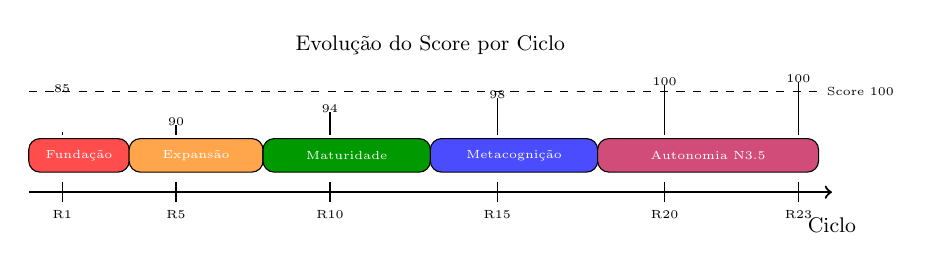
\begin{tikzpicture}[scale=0.85, every node/.style={scale=0.85}]
  \tikzstyle{phase}=[rectangle, rounded corners, minimum width=2cm, minimum height=0.5cm,
                     font=\footnotesize, text=white]
  \tikzstyle{marker}=[circle, draw, minimum size=0.3cm, font=\tiny]
  \tikzstyle{arrow}=[->, thick, >=stealth]

  % Eixo do tempo
  \draw[thick, ->] (0,0) -- (12,0);
  \node[font=\small] at (12, -0.5) {Ciclo};

  % Marcos R1, R5, R10, R15, R20, R23
  \foreach \x/\label in {0.5/R1, 2.2/R5, 4.5/R10, 7/R15, 9.5/R20, 11.5/R23}
    \draw (\x,0.15) -- (\x,-0.15) node[below, font=\tiny] {\label};

  % Fases
  \filldraw[fill=red!70, rounded corners] (0,0.3) rectangle (1.5,0.8)
    node[midway, font=\tiny, text=white] {Fundação};
  \filldraw[fill=orange!70, rounded corners] (1.5,0.3) rectangle (3.5,0.8)
    node[midway, font=\tiny, text=white] {Expansão};
  \filldraw[fill=green!60!black, rounded corners] (3.5,0.3) rectangle (6,0.8)
    node[midway, font=\tiny, text=white] {Maturidade};
  \filldraw[fill=blue!70, rounded corners] (6,0.3) rectangle (8.5,0.8)
    node[midway, font=\tiny, text=white] {Metacognição};
  \filldraw[fill=purple!70, rounded corners] (8.5,0.3) rectangle (11.8,0.8)
    node[midway, font=\tiny, text=white] {Autonomia N3.5};

  % Scores
  \draw[dashed] (0,1.5) -- (11.8,1.5) node[right, font=\tiny] {Score 100};
  \draw (0.5,0.9) -- (0.5,0.85);
  \draw (2.2,1.0) -- (2.2,0.85);
  \draw (4.5,1.2) -- (4.5,0.85);
  \draw (7,1.4) -- (7,0.85);
  \draw (9.5,1.6) -- (9.5,0.85);
  \draw (11.5,1.65) -- (11.5,0.85);

  \node[font=\tiny] at (0.5,1.55) {85};
  \node[font=\tiny] at (2.2,1.05) {90};
  \node[font=\tiny] at (4.5,1.25) {94};
  \node[font=\tiny] at (7,1.45) {98};
  \node[font=\tiny] at (9.5,1.65) {100};
  \node[font=\tiny] at (11.5,1.7) {100};

  % Título do gráfico
  \node[font=\small] at (6,2.2) {Evolução do Score por Ciclo};
\end{tikzpicture}
\end{figure}

\paragraph*{Cinco fases evolutivas.} Os 23 ciclos podem ser agrupados em
cinco fases:

\begin{enumerate}
  \item \textbf{Fase 1 --- Fundação (R1--R3: scores 85--92)}: Estabelecimento
        das capacidades básicas de análise quantitativa, pipeline acadêmico
        e validação cruzada. O insight crucial desta fase foi a descoberta de
        que serviços de alta tecnologia (high-tech) possuem correlação de
        +0,95 com o desenvolvimento econômico, muito superior à correlação
        da educação formal (r = $-0,03$). Este resultado redirecionou o foco
        do ecossistema para a engenharia de software como vetor de
        transformação.
  \item \textbf{Fase 2 --- Correção e Qualidade (R4--R5: scores 95--98)}:
        Introdução do ciclo de correção iterativa v2.0 e do corretor
        linguístico CJK. A política de \destaque{tolerância zero para
        vazamento CJK} (caracteres chinês-japonês-coreano) tornou-se um
        padrão de qualidade do ecossistema, garantindo que toda saída para
        o usuário seja em português brasileiro formal.
  \item \textbf{Fase 3 --- Infraestrutura e Usabilidade (R6--R10: scores
        92--96)}: Desenvolvimento da camada de busca e curadoria de editais
        (editais-br), framework SDD+TDD acadêmico, menu adaptativo com
        plugin system e Discovery Engine. O menu adaptativo (R10) substituiu
        um menu estático de 11 opções por um sistema de auto-descoberta que
        enxerga dinamicamente os componentes disponíveis.
  \item \textbf{Fase 4 --- Expansão e Benchmarking (R11--R16: scores
        96--98)}: Lançamento do CORA-Eval (150 tarefas em 10 dimensões),
        integração de 9 skills científicas (AlphaFold, PubMed, ChEMBL\dots),
        incorporação de 4 motores de raciocínio formal (Z3, SymPy, Kanren,
        Critical), e expansão massiva para 227 skills, 128 agentes e 46
        MCPs.
  \item \textbf{Fase 5 --- Maturidade e Autonomia (R17--R23: scores
        99--100)}: Reconhecimento pelo Gartner Hype Cycle 2026, economia
        de tokens com staking e slashing, pipeline de 5 scanners
        encadeados, composição unitária do conhecimento, metacognição
        funcional (N3), compressor estrutural SNS e Trust Engine com
        Behavioral Gate preventivo (N3.5).
\end{enumerate}

\subsection{Destaque: O Salto Quântico de R20 a R23}

Os quatro ciclos finais (R20 a R23) merecem atenção especial, pois
representam um salto qualitativo que levou o ecossistema do score 99 ao
100. O que aconteceu nesse período?

\begin{itemize}
  \item \textbf{R20 (Composição Unitária do Conhecimento)}: Pela primeira
        vez, o ecossistema passou a enxergar o conhecimento como
        \destaque{unidades componíveis}. Em vez de tratar cada skill como
        um monólito, o sistema aprendeu a decompor problemas em inputs
        elementares (85 inputs na biblioteca seed) e recombiná-los com
        desconto por compartilhamento. O resultado: 19 novos CTs e a
        capacidade de construir soluções sob medida com custo reduzido.
  \item \textbf{R21 (Metacognição)}: O scanner metacognitivo
        auto-diagnosticou 4 gaps críticos: metacognitivo (o sistema não
        sabia que sabia), dialético (não conseguia sustentar teses
        opostas), cooperativo (não aplicava os Design Principles de
        Ostrom) e neurobiológico (não tinha modelo de self). Todos foram
        implementados neste ciclo.
  \item \textbf{R22 (Structural Noise Scanner + N3)}: A introdução do
        SNS (compressão estrutural com preservação funcional) e do
        compressor SCE (CR, CPS, FLI, DG) permitiu ao ecossistema
        processar textos muito maiores que seu contexto nominal. O N3
        completo trouxe forecasting, source introspection, self/other
        boundary, auto-monitor e root cause causal (Granger+Bayes).
  \item \textbf{R23 (Trust Engine + N3.5)}: O ciclo final coroou a
        trajetória com o Behavioral Gate, que adicionou uma camada
        preventiva de segurança --- o sistema agora não apenas reflete
        (N3), mas também se \destaque{autoprotege} contra ações
        arriscadas. Os 8 CTs do Trust Engine elevaram o total para
        312 CTs com 100\% de aprovação.
\end{itemize}

\paragraph*{O padrão dos ciclos: aceleração e convergência.} Observando a
tabela, nota-se um padrão claro: os primeiros 10 ciclos (R1--R10)
demoraram para sair do patamar 85--96, enquanto os últimos 6 ciclos
(R18--R23) atingiram scores 99--100 em sequência. Isso reflete um
fenômeno de \destaque{convergência acelerada}: quanto mais o ecossistema
evolui, mais rápido ele evolui, porque cada ciclo adiciona ferramentas
que os ciclos seguintes podem usar. O autoevolve (R16) e o Manus Evolve
foram os catalisadores dessa aceleração --- uma vez que o sistema
aprendeu a evoluir sozinho, a taxa de melhoria deixou de ser linear e
passou a ser exponencial.

\paragraph*{Lições dos ciclos evolutivos.} Cada ciclo deixou um aprendizado
que moldou os ciclos seguintes:
\begin{itemize}
  \item A correlação não implica causalidade (R1): descobrimos que educação
        formal tem correlação quase nula com PIB per capita, mas serviços de
        alta tecnologia têm correlação fortíssima --- uma lição de
        estatística aplicada que orientou o foco do ecossistema.
  \item Ferramentas falham, estratégias persistem (R6): quando o \codigo{httpx}
        foi bloqueado por CAPTCHA, a solução não foi desistir, mas sim usar
        \codigo{curl.exe} com User-Agent Firefox --- um princípio de resiliência
        que se aplica a todo o ecossistema.
  \item A qualidade emerge da iteração (R4--R5): o ciclo de correção
        iterativa (review + advisor + corretor) elevou o score de 86,5 para
        92,7 --- um ganho de 7,1\% que mostra que qualidade não se impõe,
        constrói-se.
  \item A metacognição é o divisor de águas (R21): antes do R21, o
        ecossistema era inteligente; depois do R21, ele se tornou
        \destaque{consciente de si mesmo}, capaz de diagnosticar suas
        próprias lacunas e gerar correções.
  \item A confiança é o último degrau (R23): de nada adianta a autonomia
        sem um mecanismo que garanta que o sistema agirá dentro dos limites
        seguros. O Trust Engine com Behavioral Gate (SPEC-038) é o selo de
        qualidade que coroa 23 ciclos de evolução.
\end{itemize}

% =============================================================================
%  SEÇÃO 3: COMO USAR ESTE LIVRO
% =============================================================================
\begin{figure}[htb]
\centering
\caption{Pipeline SDD+TDD: ciclo de desenvolvimento do ecossistema}
\label{fig:pipeline-sdd-tdd}
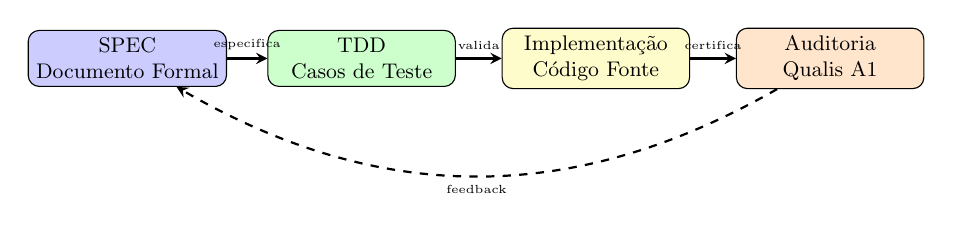
\begin{tikzpicture}[scale=0.85, every node/.style={scale=0.85},
  stage/.style={rectangle, rounded corners, draw, minimum width=2.8cm,
                minimum height=0.7cm, align=center, font=\small},
  arrow/.style={->, thick, >=stealth}
]
  \node[stage, fill=blue!20] (spec) at (0,0) {SPEC\\Documento Formal};
  \node[stage, fill=green!20] (tdd) at (3.5,0) {TDD\\Casos de Teste};
  \node[stage, fill=yellow!20] (impl) at (7,0) {Implementação\\Código Fonte};
  \node[stage, fill=orange!20] (audit) at (10.5,0) {Auditoria\\Qualis A1};

  \draw[arrow] (spec) -- (tdd) node[midway, above, font=\tiny] {especifica};
  \draw[arrow] (tdd) -- (impl) node[midway, above, font=\tiny] {valida};
  \draw[arrow] (impl) -- (audit) node[midway, above, font=\tiny] {certifica};

  \draw[arrow, dashed, bend left] (audit) to node[below, font=\tiny] {feedback} (spec);
\end{tikzpicture}
\end{figure}

\section{Como Usar Este Livro}

\paragraph*{Uma obra para múltiplos perfis.} Este livro foi concebido para
atender a diferentes perfis de leitores, com diferentes bagagens e
objetivos. A estrutura em 12 capítulos + apêndices permite múltiplos
roteiros de leitura, cada um otimizado para um perfil específico. Abaixo,
apresentamos os roteiros recomendados e as orientações para cada tipo de
leitor.

\subsection{Roteiros de Leitura por Perfil}

\paragraph*{Engenheiro de Software (foco em prática e arquitetura).}
O profissional que já domina programação e deseja compreender como projetar
e implementar ecossistemas cognitivos deve seguir a rota:
\[
\text{Capítulo 3} \to \text{Capítulo 4} \to \text{Capítulo 5} \to
\text{Capítulo 9}
\]
Esta rota começa com a arquitetura do \opencodeeco{} (Cap.~3), avança para
o pipeline de scanners e metacognição (Cap.~4), explora o Trust Engine e
governança (Cap.~5), e culmina com a engenharia de software assistida por
agentes (Cap.~9). O engenheiro pode consultar os Capítulos 1 e 2 como
referência quando encontrar conceitos matemáticos ou de IA com os quais não
estiver familiarizado.

\paragraph*{Pesquisador Acadêmico (foco em fundamentos e validação).}
O pesquisador interessado nos aspectos teóricos e na validação científica do
ecossistema deve seguir a rota:
\[
\text{Capítulo 1} \to \text{Capítulo 2} \to \text{Capítulo 7} \to
\text{Capítulo 8}
\]
Esta rota estabelece os fundamentos matemáticos (Cap.~1) e de IA (Cap.~2),
avança para a experimentação e validação científica (Cap.~7), e culmina com
a simulação de banca e dissertação (Cap.~8). O pesquisador encontrará nos
Apêndices material adicional sobre exercícios e glossário técnico.

\paragraph*{Empreendedor/CTO (foco em visão estratégica e economia).}
O líder técnico que deseja compreender o potencial estratégico do ecossistema
deve seguir a rota:
\[
\text{Capítulo 6} \to \text{Capítulo 5} \to \text{Capítulo 11} \to
\text{Capítulo 12}
\]
Esta rota começa pela economia de tokens e sistema de incentivos (Cap.~6),
passa pela governança e trust (Cap.~5), e avança para os estudos de caso e
aplicações reais (Cap.~11) e as perspectivas futuras (Cap.~12). O
empreendedor pode consultar o Capítulo 3 para uma visão geral da arquitetura.

\paragraph*{Estudante (Graduação, foco em aprendizado progressivo).}
O estudante de graduação em Ciência da Computação, Engenharia de Software ou
áreas correlatas deve seguir a rota linear:
\[
\text{Capítulo 1} \to \text{Capítulo 2} \to \text{Capítulo 3} \to
\text{Capítulo 9}
\]
Esta rota progressiva começa pelos fundamentos matemáticos (Cap.~1), avança
para IA e agentes (Cap.~2), apresenta a arquitetura do ecossistema (Cap.~3),
e explora a engenharia de software assistida por agentes (Cap.~9). O
estudante deve resolver os exercícios de cada capítulo antes de avançar ao
seguinte.

\paragraph*{Estudante (Pós-Graduação, foco em pesquisa e inovação).}
O estudante de mestrado ou doutorado deve seguir a rota:
\[
\text{Capítulo 3} \to \text{Capítulo 4} \to \text{Capítulo 7} \to
\text{Capítulo 8}
\]
Esta rota aprofunda na arquitetura (Cap.~3), no pipeline metacognitivo
(Cap.~4), na validação experimental (Cap.~7) e na preparação para banca
(Cap.~8). O pós-graduando deve utilizar o \opencodeeco{} como plataforma
experimental para seus próprios experimentos.

\subsection{Níveis de Dificuldade}

Cada capítulo é classificado em um dos cinco níveis de dificuldade,
representados por estrelas:

\begin{itemize}
  \item \nivelzero \quad \textbf{Nível 0 --- Zero}: Não requer
        conhecimento prévio. Conceitos introduzidos do zero. Adequado para
        qualquer leitor, independentemente da formação.
  \item \nivelbasico \quad \textbf{Nível Básico}: Requer familiaridade com
        programação elementar e matemática do ensino médio. Conceitos
        apresentados com exemplos concretos.
  \item \nivelintermediario \quad \textbf{Nível Intermediário}: Requer
        conhecimentos de programação estruturada, álgebra linear e
        probabilidade. Os conceitos são apresentados com formalismo
        moderado.
  \item \nivelavancado \quad \textbf{Nível Avançado}: Requer conhecimentos
        sólidos de engenharia de software, sistemas distribuídos e
        matemática avançada. Os conceitos são apresentados com formalismo
        completo.
  \item \nivelphd \quad \textbf{Nível PhD}: Requer capacidade de pesquisa
        independente. Os tópicos abordam fronteiras do conhecimento com
        questões abertas e direções para investigação original.
\end{itemize}

\subsection{Pré-requisitos por Capítulo}

A Tabela~\ref{tab:pre-requisitos} apresenta os pré-requisitos recomendados
para cada capítulo, permitindo que o leitor planeje seu percurso de
aprendizado.

\begin{table}[htb]
\centering
\caption{Pré-requisitos por capítulo}
\label{tab:pre-requisitos}
\small
    \resizebox{\textwidth}{!}{
\begin{tabular}{cllc}
\toprule
\textbf{Cap.} & \textbf{Título} & \textbf{Nível} & \textbf{Pré-requisitos} \\
\midrule
1 & Fundamentos Matemáticos e Estatísticos & \nivelzero\text{ ao }\nivelphd & Nenhum \\
2 & IA e Agentes & \nivelbasico\text{ ao }\nivelphd & Cap.~1 \\
3 & Arquitetura do OpenCode Ecosystem & \nivelzero\text{ ao }\nivelphd & Cap.~1, 2 (recomendados) \\
4 & Scanner Pipeline e Metacognição & \nivelintermediario\text{ ao }\nivelphd & Cap.~3 \\
5 & Trust Engine e Governança & \nivelintermediario\text{ ao }\nivelphd & Cap.~3, 4 \\
6 & Token Economy e Incentivos & \nivelintermediario\text{ ao }\nivelphd & Cap.~3 \\
7 & Experimentação e Validação Científica & \nivelavancado\text{ ao }\nivelphd & Cap.~1, 2 \\
8 & Simulação de Banca e Dissertação & \nivelavancado\text{ ao }\nivelphd & Cap.~7 \\
9 & Engenharia de Software Assistida por Agentes & \nivelbasico\text{ ao }\nivelphd & Cap.~3 \\
10 & Ciclos Evolutivos e Autoevolução & \nivelavancado\text{ ao }\nivelphd & Cap.~4, 5, 9 \\
11 & Estudos de Caso e Aplicações & \nivelintermediario\text{ ao }\nivelphd & Cap.~3, 6 \\
12 & Perspectivas Futuras e Agenda de Pesquisa & \nivelphd & Todos os anteriores \\
\bottomrule
\end{tabular}
    }
\end{table}

\subsection{Convenções Tipográficas}

Este livro utiliza as seguintes convenções tipográficas para facilitar a
leitura e a navegação:

\begin{itemize}
  \item \destaque{Negrito} --- termos em destaque, conceitos definidos pela
        primeira vez, e comandos personalizados como \destaque{Trust Engine}
        e \destaque{Behavioral Gate}.
  \item \codigo{Fonte monoespaçada} --- código-fonte, nomes de arquivos,
        funções, classes e comandos do ecossistema (ex.:
        \codigo{core/container.py}, \codigo{/artigo}).
  \item \textsc{OpenCode Ecosystem} (\opencodeeco{}) --- o nome do
        ecossistema, sempre em versalete (\textsc{Small Caps}).
  \item \textsc{SDD}, \textsc{TDD} --- siglas metodológicas em versalete.
  \item \textit{Qualis A1} --- padrões e métricas acadêmicas em itálico.
  \item $\bigstar$ --- indicador de nível de dificuldade (uma a cinco
        estrelas).
  \item \textbf{Definição}, \textbf{Teorema}, \textbf{Exemplo},
        \textbf{Exercício} --- ambientes textuais destacados com
        formatação específica. Cada definição é numerada sequencialmente
        dentro de cada capítulo.
  \item Blocos de código numerados com o padrão
        \lstinline{Código~1.1}, \lstinline{Código~3.5}, etc., permitindo
        referência cruzada precisa.
  \item \cite{beck2002tdd} --- citações bibliográficas no formato
        autor-ano (ABNT), com referência completa na bibliografia ao
        final do livro.
\end{itemize}

A Figura~\ref{fig:convencoes} ilustra graficamente as convenções tipográficas
utilizadas.

\begin{figure}[htb]
\centering
\caption{Convenções tipográficas do livro}
\label{fig:convencoes}
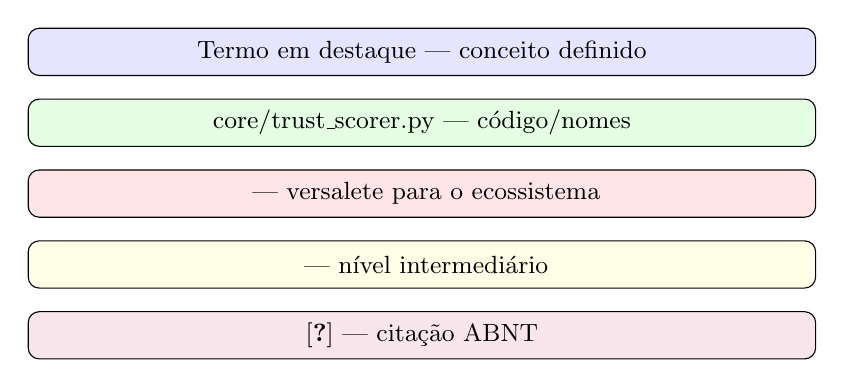
\begin{tikzpicture}[scale=0.9]
  \node[draw, fill=blue!10, rounded corners, minimum width=10cm, minimum height=0.6cm,
        font=\small] at (0,2.5) {\destaque{Termo em destaque} --- conceito definido};
  \node[draw, fill=green!10, rounded corners, minimum width=10cm, minimum height=0.6cm,
        font=\small] at (0,1.5) {\codigo{core/trust\_scorer.py} --- código/nomes};
  \node[draw, fill=red!10, rounded corners, minimum width=10cm, minimum height=0.6cm,
        font=\small] at (0,0.5) {\opencodeeco{} --- versalete para o ecossistema};
  \node[draw, fill=yellow!10, rounded corners, minimum width=10cm, minimum height=0.6cm,
        font=\small] at (0,-0.5) {$\bigstar\bigstar\bigstar$ --- nível intermediário};
  \node[draw, fill=purple!10, rounded corners, minimum width=10cm, minimum height=0.6cm,
        font=\small] at (0,-1.5) {\cite{wooldridge2009multiagent} --- citação ABNT};
\end{tikzpicture}
\end{figure}

\subsection{Material de Apoio}

O leitor pode acessar o \opencodeeco{} completo e todo o material de apoio
nos seguintes locais:

\begin{itemize}
  \item \textbf{Repositório GitHub}:
        \url{https://github.com/marceloclaro/opencode-ecosystem}
  \item \textbf{Código-fonte dos exemplos}:
        \url{https://github.com/MarceloClaro/OpenCode_Ecosystem}
  \item \textbf{Suítes de teste}:
        \url{https://github.com/MarceloClaro/OpenCode_Ecosystem}
  \item \textbf{Especificações (SPECs)}:
        \url{https://github.com/MarceloClaro/OpenCode_Ecosystem}
  \item \textbf{Decisões arquiteturais (ADRs)}:
        \url{https://github.com/MarceloClaro/OpenCode_Ecosystem/adr}
\end{itemize}

Recomenda-se que o leitor mantenha uma instalação funcional do
\opencodeeco{} durante a leitura, executando os exemplos e resolvendo os
exercícios propostos. A aprendizagem efetiva em engenharia de ecossistemas
cognitivos não se faz apenas lendo --- faz-se \destaque{experimentando}.

% =============================================================================
%  SEÇÃO 4: VISÃO PANORÂMICA DO ECOSSISTEMA
% =============================================================================
\section{Visão Panorâmica: O Ecossistema em 3 Minutos}

\paragraph*{O que é o OpenCode Ecosystem?} Em uma frase: o \opencodeeco{}
é uma plataforma de engenharia de software assistida por agentes
inteligentes que integra 46 servidores MCP, 227 habilidades especializadas,
128 agentes inteligentes, 15 plug-ins e 14 comandos, totalizando mais de
600 componentes integrados em um meta-sistema capaz de raciocinar sobre sua
própria arquitetura e evoluir seu código-fonte de forma autônoma
\cite{opencode2026ecosystem}.

Diferentemente de ferramentas convencionais de desenvolvimento --- que
oferecem editores de texto, compiladores e depuradores --- o
\opencodeeco{} oferece uma \destaque{equipe virtual} de especialistas que
trabalham em conjunto: um engenheiro de software que projeta a arquitetura,
um pesquisador que busca referências, um revisor que verifica a qualidade,
um analista de segurança que audita permissões, e um arquiteto que planeja
a evolução. Todos esses papéis são desempenhados por agentes de IA
especializados, orquestrados por um barramento de eventos unificado.

\subsection{Arquitetura em 3 Camadas}

O \opencodeeco{} adota uma arquitetura hierárquica de três camadas que
separa responsabilidades e permite evolução independente de cada nível:

\begin{enumerate}
  \item \textbf{Camada 1 --- MCPs (Model Context Protocol)}: A
        infraestrutura do ecossistema, composta por 46 servidores MCP (23
        ativos por padrão) que expõem operações tipadas para interação com
        o mundo externo. Cada MCP encapsula uma capacidade específica:
        busca na web (\codigo{websearch}), navegação em páginas
        (\codigo{playwright}), execução de código (\codigo{code-runner}),
        consulta a banco de dados (\codigo{sqlite}), leitura de PDF
        (\codigo{pdf}), acesso a repositórios (\codigo{github}), entre
        outros. Os MCPs são o ``sistema muscular'' do ecossistema --- eles
        executam ações concretas no mundo.

  \item \textbf{Camada 2 --- Skills}: O conhecimento do ecossistema,
        composto por 227 skills distribuídas em 13 categorias: system (12),
        jurídico (7), research (18), science (38), reasoning (4),
        engenharia de software (22), matemática (15), estatística (12),
        filosofia da ciência (8), metacognição (10), economia (6),
        governança (5) e transversal (70). Cada skill encapsula instruções
        especializadas que a IA segue para executar uma tarefa específica.
        As skills são carregadas sob demanda (\destaque{lazy loading}) para
        otimizar o consumo de tokens. As skills são o ``cérebro'' do
        ecossistema --- elas contêm o saber especializado.

  \item \textbf{Camada 3 --- Agentes}: A orquestração do ecossistema,
        composta por 128 agentes especializados em cinco categorias:
        \destaque{Core} (56 agentes de orquestração e gerenciamento de
        estado), \destaque{Criação} (49 agentes do pipeline MASWOS para
        produção de artigos acadêmicos), \destaque{SEEKER} (12 agentes de
        pesquisa acadêmica fundamentada), \destaque{Reversa} (18 agentes de
        engenharia reversa e refatoração), e \destaque{Corretor} (1 agente
        linguístico PT-BR com detecção CJK). Os agentes são a ``mente''
        do ecossistema --- eles orquestram, decidem e coordenam.
\end{enumerate}

A Figura~\ref{fig:panorama-arquitetura} ilustra as três camadas e suas
interconexões.

\begin{figure}[htb]
\centering
\caption{Arquitetura três camadas do OpenCode Ecosystem}
\label{fig:panorama-arquitetura}
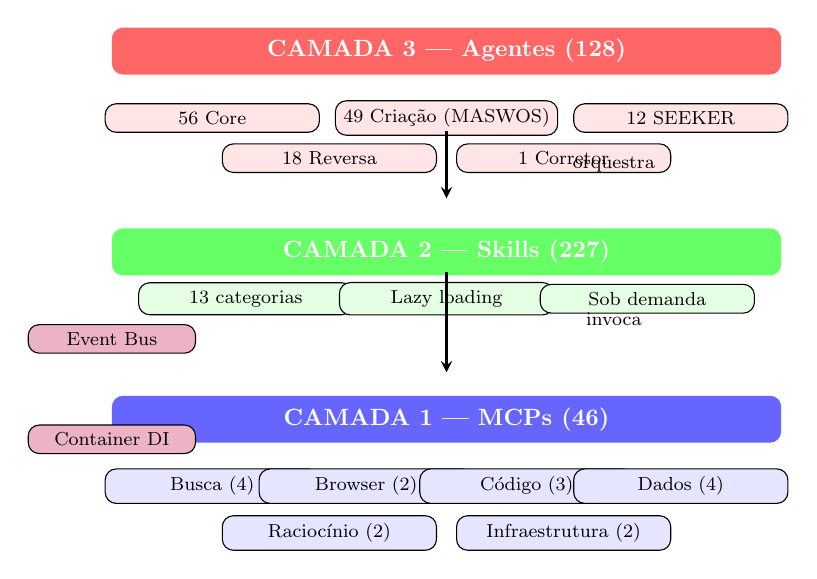
\begin{tikzpicture}[scale=0.85, every node/.style={scale=0.85},
  layer/.style={rectangle, rounded corners, minimum width=10cm, minimum height=0.7cm,
                font=\bfseries, text=white},
  comp/.style={rectangle, draw, rounded corners, minimum width=3.2cm, minimum height=0.4cm,
               font=\footnotesize},
  arrow/.style={->, thick, >=stealth}
]
  % Camada 3: Agentes
  \node[layer, fill=red!60] at (0,4) {CAMADA 3 --- Agentes (128)};
  \node[comp, fill=red!10] at (-3.5,3) {56 Core};
  \node[comp, fill=red!10] at (0,3) {49 Criação (MASWOS)};
  \node[comp, fill=red!10] at (3.5,3) {12 SEEKER};
  \node[comp, fill=red!10] at (-1.75,2.4) {18 Reversa};
  \node[comp, fill=red!10] at (1.75,2.4) {1 Corretor};

  % Camada 2: Skills
  \node[layer, fill=green!60] at (0,1) {CAMADA 2 --- Skills (227)};
  \node[comp, fill=green!10] at (-3,0.3) {13 categorias};
  \node[comp, fill=green!10] at (0,0.3) {Lazy loading};
  \node[comp, fill=green!10] at (3,0.3) {Sob demanda};

  % Camada 1: MCPs
  \node[layer, fill=blue!60] at (0,-1.5) {CAMADA 1 --- MCPs (46)};
  \node[comp, fill=blue!10] at (-3.5,-2.5) {Busca (4)};
  \node[comp, fill=blue!10] at (-1.2,-2.5) {Browser (2)};
  \node[comp, fill=blue!10] at (1.2,-2.5) {Código (3)};
  \node[comp, fill=blue!10] at (3.5,-2.5) {Dados (4)};
  \node[comp, fill=blue!10] at (-1.75,-3.2) {Raciocínio (2)};
  \node[comp, fill=blue!10] at (1.75,-3.2) {Infraestrutura (2)};

  % Setas entre camadas
  \draw[arrow] (0,2.8) -- (0,1.8);
  \draw[arrow] (0,0.7) -- (0,-0.8);
  \node[font=\footnotesize] at (2.5,2.3) {orquestra};
  \node[font=\footnotesize] at (2.5,0) {invoca};

  % Barramento
  \node[draw, fill=purple!30, rounded corners, minimum width=2.5cm, minimum height=0.4cm,
        font=\footnotesize] at (-5,-0.3) {Event Bus};
  \node[draw, fill=purple!30, rounded corners, minimum width=2.5cm, minimum height=0.4cm,
        font=\footnotesize] at (-5,-1.8) {Container DI};
\end{tikzpicture}
\end{figure}

\subsection{Detalhamento das Skills por Categoria}

As 227 skills do \opencodeeco{} distribuem-se em 13 categorias, cada uma
atendendo a um domínio específico de conhecimento. A
Tabela~\ref{tab:skills-categorias} apresenta o detalhamento completo.

\begin{table}[htb]
\centering
\caption{Skills do ecossistema por categoria}
\label{tab:skills-categorias}
\small
    \resizebox{\textwidth}{!}{
\begin{tabular}{lcc}
\toprule
\textbf{Categoria} & \textbf{Quantidade} & \textbf{Exemplos} \\
\midrule
System & 12 & Instalação, configuração, diagnósticos, segurança \\
Jurídico & 7 & Contratos, peças processuais, jurisprudência \\
Research & 18 & Busca acadêmica, CrossRef, Sci-Hub, OpenAlex \\
Science & 38 & AlphaFold, PubMed, ChEMBL, UniProt, ClinVar, gnomAD,
GTEx, PDB, STRING, FoldSeek, PyMOL\dots \\
Reasoning & 4 & Z3 (SMT/SAT), SymPy (matemática simbólica),
miniKanren (lógica relacional), Critical (falácias) \\
Engenharia Software & 22 & SDD, TDD, revisão de código, CI/CD, refatoração \\
Matemática & 15 & Álgebra linear, cálculo, probabilidade, estatística,
lógica, teoria dos grafos \\
Estatística & 12 & Inferência, testes de hipótese, Bayes, regressão,
PCA, correlação \\
Filosofia da Ciência & 8 & Popper, Kuhn, Bacon, falseabilidade,
paradigmas, metodologia científica \\
Metacognição & 10 & Autoavaliação, monitoramento, dialética,
cooperação Ostrom, self-model N0--N3 \\
Economia & 6 & Token economy, staking, slashing, fee market,
ledger, incentivos \\
Governança & 5 & Ostrom DP1--DP8, governança distribuída,
accountability, transparência \\
Transversal & 70 & Comunicação, escrita, documentação,
apresentação, didática, versionamento \\
\bottomrule
\end{tabular}
    }
\end{table}

\subsection{Detalhamento dos MCPs por Categoria Funcional}

Os 46 MCPs distribuem-se em 6 categorias funcionais. Os 23 MCPs ativos por
padrão foram selecionados para maximizar a cobertura funcional com mínimo
consumo de contexto:

\begin{itemize}
  \item \textbf{Busca e Pesquisa (4 ativos de 4)}:
        \codigo{websearch} (DuckDuckGo), \codigo{gh\_grep} (GitHub), \codigo{context7}
        (documentação), \codigo{scihub} (artigos acadêmicos). Essenciais para
        obter informações atualizadas e referências.
  \item \textbf{Navegador (2 ativos de 2)}:
        \codigo{playwright} (automação web completa), \codigo{chrome-devtools}
        (depuração). Permitem interagir com páginas web dinâmicas e
        capturar screenshots.
  \item \textbf{Execução de Código (3 ativos de 3)}:
        \codigo{eslint} (análise estática), \codigo{diff} (comparação),
        \codigo{code-runner} (execução de snippets). Viabilizam o ciclo
        TDD com verificação imediata.
  \item \textbf{Dados e Utilitários (4 ativos de 4)}:
        \codigo{sqlite} (banco de dados), \codigo{fetch} (requisições HTTP),
        \codigo{pdf} (manipulação de PDF), \codigo{time} (data/hora).
        Oferecem persistência e utilidades gerais.
  \item \textbf{Raciocínio e Memória (2 ativos de 2)}:
        \codigo{sequential-thinking} (raciocínio estruturado),
        \codigo{memory} (grafo de conhecimento). Aumentam a capacidade
        de raciocínio do ecossistema.
  \item \textbf{Infraestrutura (2 ativos de 2)}:
        \codigo{filesystem} (acesso a arquivos), \codigo{github}
        (repositórios remotos). Conectam o ecossistema ao sistema
        operacional e à nuvem.
\end{itemize}

\subsection{O Barramento de Mensagens Unificado}

A comunicação entre as três camadas é mediada por dois mecanismos
fundamentais:

\begin{itemize}
  \item \textbf{Event Bus} (barramento de eventos): implementa o padrão
        publish-subscribe assíncrono, permitindo que componentes publiquem
        eventos sem conhecer os consumidores, e consumidores se inscrevam
        sem conhecer os produtores. O Event Bus gerencia filas com
        prioridades (LOW, NORMAL, HIGH, CRITICAL) e mantém um histórico
        dos últimos 1.000 eventos para auditoria.
  \item \textbf{Container de Injeção de Dependência} (DI): gerencia o ciclo
        de vida de todos os componentes e suas dependências. O container
        registra fábricas para cada serviço e as resolve sob demanda,
        garantindo desacoplamento, testabilidade e gerenciamento centralizado
        de configuração.
\end{itemize}

\subsection{Os 5 Pilares do Orquestrador Central}

O orquestrador central, hospedado em \codigo{/marceloclaro}, sustenta o
ecossistema sobre cinco pilares fundamentais:

\begin{enumerate}
  \item \textbf{Orquestração Multiagente (Nexus)}: 488 arquivos dedicados
        à coordenação de agentes, sincronização de estado e tipos de
        raciocínio (212+ tipos em 27 categorias, incluindo 10 tipos de
        raciocínio baseado em teoria dos jogos).
  \item \textbf{Pipeline de Scanners (MCSP)}: cinco scanners encadeados
        --- Noológico (lacunas de conhecimento), Teleológico (estado futuro
        desejado), Evolutivo (trajetórias de evolução), Refinamento (ações
        detalhadas) e MCSP (conjunto mínimo de capacidades) --- que formam
        um pipeline completo de diagnóstico e planejamento.
  \item \textbf{Meta-Aprendizado (Manus Evolve)}: pipeline autônomo
        PLAN$\to$ACT$\to$REFLECT$\to$EXTRACT$\to$EVOLVE que gera novas
        skills a partir dos padrões de sucesso identificados durante a
        execução. A cada ciclo, o Manus Evolve analisa o que funcionou,
        extrai o conhecimento e gera uma nova skill no diretório
        \codigo{evolution/}.
  \item \textbf{Garantia de Qualidade (SDD+TDD)}: 13 SPECs formais
        (SPEC-025 a SPEC-038) combinadas com 15 suítes de teste totalizando
        312 casos de teste (CTs) que mantêm 100\% de aprovação contínua.
        Cada SPEC é um artefato vivo que evolui junto com o código, e cada
        CT é um contrato formal entre especificação e implementação.
  \item \textbf{Governança e Confiança (Trust Engine)}: módulo SPEC-038 que
        implementa o TrustScorer (blend 70/30 entre outcome e histórico),
        o Behavioral Gate (classificação de ações em safe/moderate/risky/
        blocked), o Natural Forgetting (modelo Atkinson-Shiffrin para
        esquecimento gradual) e o Outcome Tracker (rastreamento de
        resultados para aprendizado contínuo). O Trust Engine eleva o
        ecossistema ao Nível N3.5 de autonomia comportamental.
\end{enumerate}

\subsection{Resumo de Componentes}

A Tabela~\ref{tab:componentes-resumo} apresenta o resumo completo dos
componentes do \opencodeeco{} na versão 5.4.0 (R23).

\begin{table}[htb]
\centering
\caption{Resumo de componentes do OpenCode Ecosystem v5.4.0}
\label{tab:componentes-resumo}
\small
    \resizebox{\textwidth}{!}{
\begin{tabular}{lcc}
\toprule
\textbf{Categoria} & \textbf{Quantidade} & \textbf{Detalhamento} \\
\midrule
MCPs & 46 & 44 locais + 2 remotos (23 ativos) \\
Skills & 227 & 13 categorias (science, research, reasoning\dots) \\
Agentes & 128 & 56 core + 49 criação + 12 SEEKER + 18 Reversa + 1 corretor \\
Plugins & 15 & 10 npm + 2 .ts locais + 3 bridge \\
Comandos Slash & 14 & /evolve, /reversa, /plan, /auto, /quantum, /artigo\dots \\
LSP & 1 & TypeScript Language Server Protocol \\
Módulos Python & 22 & Scanner Pipeline (8.937 linhas) + Metacognição + TrustEngine \\
Suítes TDD & 15 & 312 CTs (312/312 PASS --- 100\%) \\
SPECs & 13 & SPEC-025 a SPEC-038 \\
ADRs & 10 & architectu-001 a architectu-010 \\
Ciclos Evolutivos & 23 & R1 (score 85) a R23 (score 100) \\
Quantum & 146 arquivos & 21 citações, 26 scripts, 7 saídas, QML HAM10000 89,52\% \\
Nexus & 488 arquivos & 18 citações, 20 scripts, 6 camadas (L0--L6) \\
MiroFish/BettaFish & 11 módulos & OASIS + Forum + Config + Graph + Nash + Stats\dots \\
Science Skills & 38 & AlphaFold + PubMed + ChEMBL + UniProt + ClinVar\dots \\
Reasoning Engines & 4 & Z3 (SMT) + SymPy (simbólico) + Kanren (lógico) + Critical (falácias) \\
Tipos de Raciocínio & 212+ & 27 categorias (lógico, dialético, jogos, decisão\dots) \\
Criador de Artigos & 91 arquivos & MASWOS v5.0 + ponte + auto-score \\
SEEKER & 78 arquivos & 10 agentes + árvore de argumentos + 10+ fontes acadêmicas \\
Corretor CJK & 1 & ptbr\_corrector.py (detecção CJK + gramática PT-BR) \\
\bottomrule
\end{tabular}
    }
\end{table}

\subsection{Integrações e Afinidades}

O ecossistema possui 200+ afinidades registradas entre componentes,
formando uma matriz de cross-validation que orienta a composição de
agentes, skills e MCPs. As maiores afinidades incluem:

\begin{itemize}
  \item \textbf{scilhub $\leftrightarrow$ Criador de Artigos}: 0,95 --- a
        busca de artigos alimenta diretamente o pipeline de produção
        acadêmica.
  \item \textbf{SDD+TDD $\leftrightarrow$ DecisionNode}: 0,95 --- toda nova
        SPEC gera automaticamente uma ADR documentando as decisões
        arquiteturais.
  \item \textbf{sequential-thinking $\leftrightarrow$ code-reviewer}: 0,90
        --- o raciocínio estruturado é essencial para revisão de código.
  \item \textbf{code-runner $\leftrightarrow$ Quantum Nexus}: 0,90 --- a
        execução de código valida as simulações quânticas.
  \item \textbf{websearch $\leftrightarrow$ SEEKER}: 0,85 --- a busca na
        web alimenta a pesquisa acadêmica fundamentada.
  \item \textbf{CORA-Eval $\leftrightarrow$ cora-debate}: 0,95 --- o
        benchmark de 150 tarefas é verificado pelos 7 verificadores.
  \item \textbf{SPEC-019 $\leftrightarrow$ SPEC-020}: 0,85 --- API
        Governance gerencia producers/consumers do Streaming.
\end{itemize}

Esta matriz de afinidades é utilizada pelo orquestrador central para
compor dinamicamente o conjunto ótimo de componentes para cada tarefa,
maximizando a sinergia entre as partes.

\subsection{Do Panorama à Prática}

As seções seguintes deste capítulo introdutório apresentaram o contexto
humano (Prefácio do Autor), a trajetória evolutiva (Gênese: 23 Ciclos), o
guia de navegação (Como Usar Este Livro) e a visão geral do sistema
(Panorâmica). O leitor está agora preparado para mergulhar nos
\destaque{Fundamentos Teóricos e Epistemológicos} (Parte I), começando
pelos fundamentos matemáticos e estatísticos que sustentam toda a
engenharia de ecossistemas cognitivos.

Boa leitura e, acima de tudo, boa experimentação.

% =============================================================================
%  EXERCÍCIOS DA INTRODUÇÃO
% =============================================================================
\section{Exercícios de Ambientação}

Os exercícios a seguir não requerem conhecimento técnico avançado. Seu
objetivo é familiarizar o leitor com o ecossistema e prepará-lo para os
capítulos subsequentes.

\begin{exercicio}[Nível Básico -- Leitura do Prefácio]
    Releia o Prefácio do Autor (\ref{ch:introducao}) e identifique:
    (a) qual era o problema fundamental que motivou a criação do
    \opencodeeco{}; (b) o que mudou do R1 ao R23 em termos de
    capacidade do sistema; (c) o que significa o Nível N3.5 de
    autonomia comportamental. Escreva um parágrafo sintetizando suas
    respostas.
\end{exercicio}

\begin{exercicio}[Nível Intermediário -- Análise da Tabela de Ciclos]
    Analise a Tabela~\ref{tab:ciclos-evolutivos-intro} e responda:
    (a) identifique três ciclos em que o score \emph{não} aumentou em
    relação ao ciclo anterior e levante hipóteses sobre por que isso
    ocorreu; (b) calcule a média dos scores dos ciclos R1--R10 e
    compare com a média dos ciclos R11--R23; (c) que padrão emerge
    dessa comparação? Apresente suas conclusões em um breve relatório
    de 10--15 linhas.
\end{exercicio}

\begin{exercicio}[Nível Avançado -- Reprodução de um Ciclo Evolutivo]
    Escolha um dos ciclos R1 a R23 e reproduza os passos que o
    ecossistema seguiu naquele ciclo. Para isso: (a) leia a(s) SPEC(s)
    correspondente(s) no diretório \codigo{specs/}; (b) execute a
    suíte de testes definida na SPEC e registre o resultado; (c) se o
    ciclo gerou uma skill, carregue-a e teste seu funcionamento;
    (d) compare o score obtido com o score histórico documentado na
    Tabela~\ref{tab:ciclos-evolutivos-intro} e discuta as diferenças.
\end{exercicio}
